\section{Case Study}
\label{sec:case}

%%\wrm{Re-do case studies in Bud} \wrm{Break cart development down into
%%iterations} \wrm{How does the language naturally lead us to an order
%%independent style?  Talk about inserting all sorts of exotic stuff like queues
%%if we want a highly order-dependent imperative style.}

\begin{comment}

\jmh{We discussed the following on the phone.  (1) Handle shopping in two styles: destructive updates, and disorderly accumulation of increment/decrement.  (2) Do analysis on them to detect need for coordination in only the first, show that (annotated) 2PC removes the compiler warning.  (3) Deploy destructive+2PC on EC2 and show practical benefits of avoiding coordination.  (4) Evolve the program with new rules for checkout and/or inventory, show how the disorderly version is no longer monotonic.  Fix that  with 2PC where needed.  Also make sure the destructive version works with the new rules.  Now show that the disorderly version is still better than the destructive one, by coordinating only where needed.}

\jmh{Finally, show what would happen if you didn't coordinate the inventory bit, but tracked taint.  Note that tainted output is the stuff where programmers need to write compensation logic.}

\end{comment}

%%In this section, we implement two different styles of distributed shopping cart
%%applications in Bud.  First, we implement a ``destructive,'' overwriting
%%shopping cart application using a simple key-value store implemented in Bud.
%%Second, we implement a ``disorderly'' cart which accumulates updates in a 
%%set-wise fashion and describes how to combine the updates into a final result.

Figure~\ref{fig:pdg-destructive} shows a Bud implementation of a shopping
cart built on a key-value store abstraction.  Each cart (identified by a
session identifier) is associated with a key, whose value is a Ruby array
representing the set of items contained in the cart at any time.  The 
scratch table \emph{kvstore} is defined by the KeyValueStore module (not shown), 
which the shopping cart extends via Ruby inheritance, and is used in a manner
analogous to the \emph{put} function for hash tables.  

Cart updates are transmitted from the client in line 28,
thereafter appearing in the \emph{action\_msg} collection at a server replica.
For each such arriving tuple,
line 2 probes the \emph{bigtable} collection for a matching
session.  If found, lines 2-6 are evaluated; otherwise the join conditions
in lines 10-11 will be met and lines 12-18 will instead be evaluated.
In the first case, both the key and a singleton array value must be created.
In the second, the old copy of the array must be modified to produce a new 
value, which replaces the original array stored under the session key.
Finally, when a checkout message is received, value in \emph{bigtable}
associated with the given session is extracted (via the join on lines 22-23)
and sent back to the client.

Figure~\ref{fig:} shows an alternative shopping cart implementation, in which
updates are accumulated in a disorderly fashion and summarized only at 
checkout.  Line 0 appends all client updates to the persistent table 
\emph{cart\_action}.  Lines 2-3 define \emph{action\_cnt} as an aggregate
over \emph{cart\_action}, in the style of an SQL group-by statement: for
each item associated with a cart, we could the number of times it was added
or deleted.  Lines 11-16 define the collection \emph{status} as a 3-way
join between the \emph{checkout} message and two copies of 
\emph{action\_cnt} (one corresponding to additions and one to deletions),
and for each item, compute it quantity as the different of the two counts
in line 14.  A \emph{response} message containing the quantity is then sent 
to the client in lines 18-22.  Because the disorderly implementation does not
use a separate storage system, it must replicate its own state to replicas 
via multicast (lines 24-26).


\begin{figure}[t]
\begin{tiny}
\begin{verbatim}

0: kvstore <= action_msg.map do |a|
1:   unless bigtable.map{|b| b.key}.include? a.session
2:     if a.action == "A"
3:       [a.server, a.client, a.session, a.reqid, [a.item]]
4:     elsif a.action == "D"
5:       [a.server, a.client, a.session, a.reqid, []]
6:     end
7:   end
8: end
9: 
10: kvstore <= join([bigtable, action_msg]).map do |b, a|
11:   if b.key == a.session
12:     if a.action == "A"
13:       [a.server, a.client, a.session, a.reqid, b.value.push(a.item)]
14:     elsif a.action == "D"
15:       copy = b.value.clone;
16:       copy.delete_at(copy.index(a.item));
17:       [a.server, a.client, a.session, a.reqid, copy]
18:     end
19:   end
20: end
21:
22: response_msg <+ join([bigtable, checkout_msg]).map do |s, c|
23:   if s.key == c.session
24:     [c.client, c.server, s.key, s.value]
25:   end
26: end
27: 
28: action_msg <+ client_action.map{|a| a}


\end{verbatim}
\end{tiny}
\centering
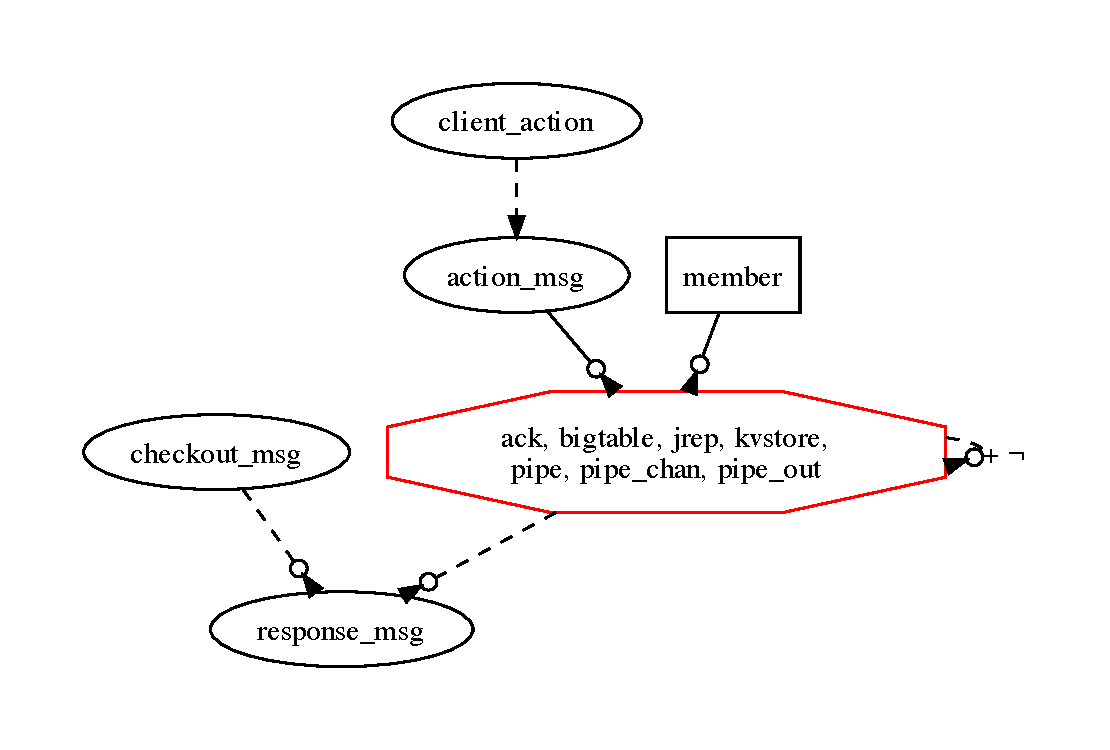
\includegraphics[width=0.9\linewidth]{fig/destructive.pdf}

\caption{Destructive Cart (cycles collapsed)}
\label{fig:pdg-destructive}
\end{figure}


\subsection{Analysis}


For each cart, we apply whole-program analysis techniques to discover points of 
order.  The Bud interpreter automatically generates
a graphical representation of the dependency graph of collections 
(and hence the 
flow of tuples) as a staged dataflow.  Each node in the graph is either
a collection or a cluster of collections (as described below).  
Asynchronous messaging
is indicated by a dashed line in the graph, while edges that involve 
nonmonotonic logic are marked with a $\lnot$.  Edges that involve a temporal 
edge are marked with a $+$.  Strongly connected components having both a $\lnot$ and a $+$ edge are grouped into temporal clusters.  
%%Individual monotonic components 
%%(or strata) are surrounded by a dotted rectangle.  A point of order occurs
%%wherever an edge crosses strata, or at any self-edge attached to a temporal cluster.
Points of order are indicated by lightning bolts.

To resolve a point of order, the programmer may add coordination logic.
Instead of reanalyzing the augmented program, we associate coordination code
with an annotation that can
be interpreted as a contract about a point of order.  Such contracts will
typically guarantee an ordering over arriving tuples, or guarantee a 
a barrier-passing condition (e.g., indicating that there will be no more tuples).

It should be intuitively obvious that the ``destructive'' cart based on
array mutation is nonmonotonic and potentially sensitive to the order
of its inputs.
And indeed, the graph in Figure~\ref{fig:pdf-destructive}
indicates that there are
points of order between \emph{iaction} and the temporal cluster
and between the temporal cluster and itself.  This means that the arrival 
timing and order of both client updates (via \emph{iaction}) and
server replication (via the meta-edge in the temporal cycle from 
\emph{kvstore} to itself) may result in different
end results.  Although there is no syntactically obvious nonmonotonicity in the destructive
cart code as shown, the underlying key-value store uses updateable state
to implement the storage of opaque, mutable values of 
keys~\footnote{Our full-length paper expands the SCC to analyze the
key-value store in detail}, 
and our global analysis detects this.
To ensure a consistent final state across all replicas, we may require coordination
between client and server at every update to the cart, and between the 
server and all replicas at each update.  

We can easily achieve coordination without modfying the cart implementation
by redefining the key-value store to extend
a reliable or quorum-based delivery module instead of the best-effort module
that the basic key-value store extends, and require acknowledgement from a server or a quorum of servers, respectively.
The simplest (and least performant) approach is to require unanimous quorum,
approximating ``eager replication''~\cite{dangers} via two-phase commit.

Of course, eager replication substantially decreases system throughput.  
%%One is tempted
%%to argue that we can simply use best-effort, asynchronous delivery,
%%because although we use an ordered data structure (an array) and nonmonotonic
%%operations (updating values in the store), the order of operations on the array
%%affects only the ordering of its contents, not the set of elements it contains.
Because we only care about the set of elements contained in the value array
and not its order, we might be tempted to argue that 
the shopping cart application is eventually consistent
when asynchronously updated, and forgo the synchronization.  Unfortunately, such informal reasoning can
hide serious bugs: consider what happens if a delete update is received
before the addition it was intended to cancel.



\begin{figure}[t]
\begin{tiny}
\begin{verbatim}
0:  cart_action <= action.map { |c| [c.session, c.item, c.action, c.reqid] }
1:
2:  action_cnt <= cart_action.group([cart_action.session, 
3:    cart_action.item, cart_action.action], count(cart_action.reqid))
4:
5:  action_cnt <= cart_action.map do |a| 
6:    unless cart_action.map{|c| [c.session, c.item] if c.action == "D"}.include? [a.session, a.item] 
7:      [a.session, a.item, 'D', 0]
8:    end 
9:  end
10: 
11: status <= join([action_cnt, action_cnt, checkout]).map do |a1, a2, c| 
12:   if a1.session == a2.session and a1.item == a2.item 
13:   and a1.session == c.session and a1.action == "A" and a2.action == "D"
14:     [a1.session, a1.item, a1.cnt - a2.cnt] if (a1.cnt - a2.cnt) > 0
15:   end
16: end
17:
18: response <= join([status, checkout]).map do |s, c| 
19:   if s.session == c.session
20:     [c.client, c.server, s.session, s.item, s.cnt]
21:   end
22: end
23: 
24: action <+ join([action, member]).map do |a, m|
25:   [m.player, a.server, a.session, a.item, a.action, a.reqid]
26: end


\end{verbatim}
\end{tiny}

\centering
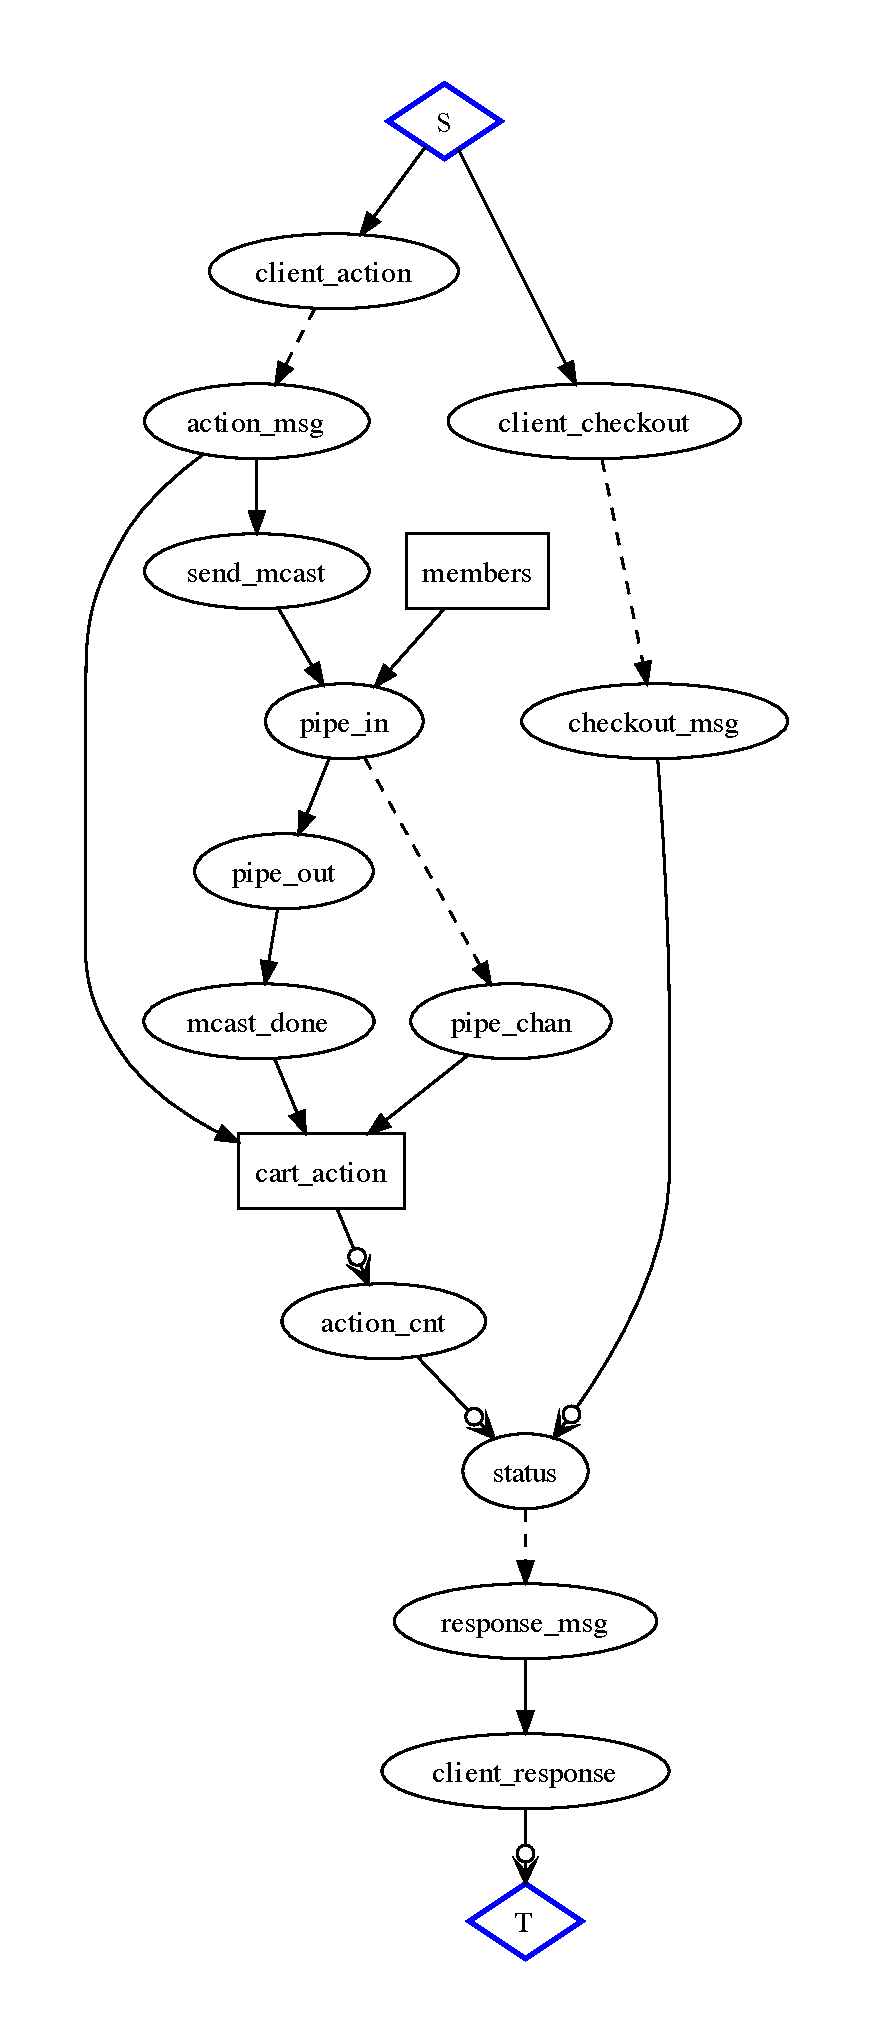
\includegraphics[width=0.7\linewidth]{fig/disorderly.pdf}
\caption{Disorderly Cart}
\label{fig:pdg-disorderly}
\end{figure}


Figure~\ref{fig:pdg-disorderly} presents a ``disorderly'' cart implementation
and analysis.  In this top-down rewrite, we model the state shopping cart 
as the set of changes in each session, rather than as a mutable cell in a
key-value abstraction.  By doing so we enable our analysis to recognize the
inherent commutativity of basic set operations, and flag most of the 
program logic as consistent without coordination.

Dotted lines indicate that 
\emph{action} (owned by the server) is derived from \emph{client\_action} 
(owned by the client) via an asynchronous message, and that \emph{action} 
derives itself via messages when it is replicated.  However, the analysis
shows that because these derivations are strictly monotonic, no points of
order are crossed.  Hence, clients may send and servers may replicate 
updates without any coordination: regardless of timing and ordering, the end
result will be the same.

The analysis does indicate a point of order at checkout, when a \emph{checkout}
message is joined with an aggregate over the set of updates.  While the 
accumulation of state has been monotonic, summarization of the cart state
requires us to assume (or prove) that there will be no further updates.
Consider a checkout message and a final update message racing from a client
to one of the replicas: the order in which they arrive will surely affect
the contents of the response message.  

Unlike in our previous implementation, which discovered a point of order at
every update and replication step, the current analysis has indicated
a point of order at checkout.  We need only coordinate once per session to
ensure that the response to the client is deterministic.


